\section{Extending the assumptions of bunching}

The bunching estimator developed in Section~1 relies on two central pillars: frictionless re-optimization around the statutory kink and the ability to reconstruct the unobserved counterfactual income density $g(z)$ across the excluded region. This section examines both assumptions formally. Part~(i) introduces contract-renegotiation frictions into a stylized quasilinear economy \parencite{chetty2011adjustment} and characterizes the resulting attenuation bias in the Saez-style elasticity estimator $\hat{\epsilon}$. Part~(ii) turns to counterfactual identification, develops two nonparametric alternatives to global polynomial extrapolation, illustrates them in the $(z, g(z))$ plane, and explains why bunching analyses should report identified intervals rather than single point estimates.\footnote{While Appendix~A derives the baseline elasticity formula~\eqref{eq:elasticity} for a general ability distribution without frictions ($\phi = 0$), Part~(i.1) below specializes that frictionless benchmark to a unit-mass uniform ability economy to obtain an exact closed-form counterfactual $g(z)$ and set up the new extensions in Parts~(i.2) and~(ii): adjustment frictions ($\phi > 0$), attenuation bias, and alternative counterfactual bounds.}

\subsection*{(i) Frictions, excess mass, and attenuation bias}

Consider a continuum of agents of unit mass whose unobserved ability $n > 0$ is uniformly distributed on $[\underline{n}, \overline{n}] \subset \mathbb{R}_{++}$, so that the ability probability density function is
\begin{equation}
f_N(n) = \frac{1}{\overline{n} - \underline{n}}, \qquad n \in [\underline{n}, \overline{n}],
\label{eq:p2_ability_pdf}
\end{equation}
and $f_N(n) = 0$ outside $[\underline{n}, \overline{n}]$, satisfying $\int_{\underline{n}}^{\overline{n}} f_N(n)\,dn = 1$. Agents have quasilinear, isoelastic preferences over consumption $c$ and hours worked (equivalently, pre-tax taxable income when the wage rate is normalized to unity) $z \ge 0$:
\begin{equation}
u(c, z) = c - \frac{n^{-1/\epsilon}}{1 + 1/\epsilon}\,z^{1 + 1/\epsilon},
\label{eq:p2_utility}
\end{equation}
where $\epsilon > 0$. Under a piecewise-linear tax schedule with a convex kink at $z^* \in \big[\underline{n}(1-\tau_0)^\epsilon,\; \overline{n}(1-\tau_1)^\epsilon\big]$ and marginal rates $0 \le \tau_0 < \tau_1 < 1$,\marginnote{A convex tax kink ($\tau_1 > \tau_0$) lowers the marginal return to work from $1-\tau_0$ to $1-\tau_1$ at $z^*$, inducing upper-tail taxpayers to bunch downward at $z^*$.} disposable consumption is given by
\begin{equation}
c(z) = \begin{cases}
(1-\tau_0)z & \text{if } z < z^*, \\[3pt]
(1-\tau_0)z^* + (1-\tau_1)(z - z^*) & \text{if } z \ge z^*.
\end{cases}
\label{eq:p2_budget}
\end{equation}
Renegotiating an existing labor contract from $z_0$ to a new level $z_1$ entails a fixed utility adjustment cost $\phi \ge 0$, so a worker re-optimizes if and only if
\begin{equation}
u\big(c(z_1), z_1\big) - u\big(c(z_0), z_0\big) > \phi.
\label{eq:p2_friction_rule}
\end{equation}

\subsubsection*{1. Frictionless benchmark ($\phi = 0$)}

To evaluate how optimization frictions distort the Saez-style elasticity estimator $\hat{\epsilon}$, we first need an exact, closed-form benchmark of the economy without frictions ($\phi = 0$). Because empirical bunching formulas relate observed clustering in taxable income $z$ to the unobserved counterfactual density $g(z)$, solving the frictionless problem serves two purposes: it pins down each agent's baseline income choice $z_0(n)$ as a function of latent ability $n$, and it translates the exogenous ability distribution $f_N(n)$ into the exact counterfactual income density $g(z)$ that would prevail in the absence of the kink.

In the counterfactual economy without a kink, every peso is taxed at the constant marginal rate $\tau_0$, so disposable consumption is $c(z) = (1-\tau_0)z$ for all $z \ge 0$. An agent of ability $n$ chooses $z$ to solve
\begin{equation}
\max_{z \ge 0} \; (1-\tau_0)z - \frac{n^{-1/\epsilon}}{1 + 1/\epsilon}\,z^{1 + 1/\epsilon}.
\end{equation}
Because the objective is strictly concave in $z$ ($\partial^2 u / \partial z^2 = -\frac{1}{\epsilon} n^{-1/\epsilon} z^{1/\epsilon - 1} < 0$ for all $z > 0$) and the marginal disutility at $z = 0$ is zero while $1-\tau_0 > 0$, the first-order condition is both necessary and sufficient for a unique interior optimum:
\begin{equation}
\frac{\partial u}{\partial z} = (1-\tau_0) - n^{-1/\epsilon} z^{1/\epsilon} = 0
\quad\Longleftrightarrow\quad
z^{1/\epsilon} = n^{1/\epsilon}(1-\tau_0)
\quad\Longleftrightarrow\quad
z_0(n) = n(1-\tau_0)^\epsilon.
\label{eq:p2_z0}
\end{equation}

We can now recover the counterfactual income density $g(z)$ directly from the cumulative distribution function (CDF) of optimal earnings. Since $z_0(n)$ is strictly increasing in ability, an agent earns at most $z$ if and only if their ability satisfies $n \le z(1-\tau_0)^{-\epsilon}$. Using the uniform ability distribution~\eqref{eq:p2_ability_pdf} over $[\underline{n}, \overline{n}]$, the counterfactual income CDF $G(z) \equiv \mathbb{P}(Z_0 \le z)$ is
\begin{equation}
G(z) = \mathbb{P}\!\left(N \le z(1-\tau_0)^{-\epsilon}\right)
= \int_{\underline{n}}^{z(1-\tau_0)^{-\epsilon}} \frac{1}{\overline{n}-\underline{n}}\,dn
= \frac{z(1-\tau_0)^{-\epsilon} - \underline{n}}{\overline{n}-\underline{n}},
\end{equation}
for any $z \in \big[\underline{n}(1-\tau_0)^\epsilon,\; \overline{n}(1-\tau_0)^\epsilon\big]$ (with $G(z) = 0$ below the lower bound and $G(z) = 1$ above the upper bound). Differentiating $G(z)$ with respect to $z$ yields the counterfactual probability density function:
\begin{equation}
g(z) = G'(z) = \frac{1}{(\overline{n}-\underline{n})(1-\tau_0)^\epsilon},
\qquad z \in \big[\underline{n}(1-\tau_0)^\epsilon,\; \overline{n}(1-\tau_0)^\epsilon\big],
\label{eq:p2_gz}
\end{equation}
and $g(z) = 0$ otherwise. Integrating~\eqref{eq:p2_gz} over its support confirms $\int_{\underline{n}(1-\tau_0)^\epsilon}^{\overline{n}(1-\tau_0)^\epsilon} g(z)\,dz = 1$. Notice that because ability is uniform and $z_0(n)$ is linear in $n$, $g(z)$ is constant across its support (Figure~\ref{fig:p2_uniform_density}).\footnote{\texttt{code: source/plots/p2.py:L194}}\marginnote{Uniform ability combined with isoelastic disutility makes $g(z)$ exactly constant, eliminating local-uniformity approximation error.}

\begin{figure}[htbp]
\centering
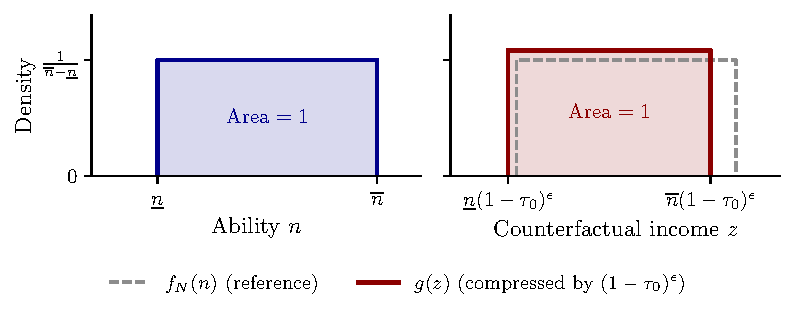
\includegraphics[width=0.92\textwidth]{p2_uniform_density.pdf}
\caption{Stylized uniform ability density $f_N(n)$ (left) and the induced counterfactual income density $g(z)$ (right). Compressing the support by $(1-\tau_0)^\epsilon$ scales the constant density height up by $(1-\tau_0)^{-\epsilon}$ so total mass remains equal to one.}
\label{fig:p2_uniform_density}
\end{figure}

Having characterized the counterfactual income distribution $g(z)$ in the absence of the kink, we now introduce the piecewise-linear tax schedule~\eqref{eq:p2_budget} while maintaining $\phi = 0$. Our goal is to determine which ability types relocate to the kink $z^*$ and to map that set of agents into an exact expression for the excess mass $B$. Substituting $c(z)$ into~\eqref{eq:p2_utility} yields the piecewise objective $U(z; n) \equiv u(c(z), z)$:
\begin{equation}
U(z; n) = \begin{cases}
(1-\tau_0)z - \dfrac{n^{-1/\epsilon}}{1 + 1/\epsilon}\,z^{1 + 1/\epsilon} & \text{if } z < z^*, \\[8pt]
(1-\tau_0)z^* + (1-\tau_1)(z - z^*) - \dfrac{n^{-1/\epsilon}}{1 + 1/\epsilon}\,z^{1 + 1/\epsilon} & \text{if } z \ge z^*.
\end{cases}
\end{equation}
Because $c(z)$ is continuous and concave (its slope drops discretely from $1-\tau_0$ to $1-\tau_1$ at $z^*$) and the disutility term is strictly convex and continuously differentiable, $U(z; n)$ is strictly concave on $[0, \infty)$ and differentiable everywhere except at the kink $z^*$. On the upper branch ($z > z^*$), an interior first-order condition gives $(1-\tau_1) - n^{-1/\epsilon}z^{1/\epsilon} = 0$, implying an unconstrained upper-bracket choice of $z_1(n) = n(1-\tau_1)^\epsilon$. At the threshold $z^*$ itself, however, the objective exhibits a corner; thus, optimality is governed not by a zero-derivative condition, but by comparing the left- and right-hand directional derivatives:
\begin{equation}
U_-'(z^*; n) = (1-\tau_0) - \left(\frac{z^*}{n}\right)^{1/\epsilon},
\qquad
U_+'(z^*; n) = (1-\tau_1) - \left(\frac{z^*}{n}\right)^{1/\epsilon}.
\label{eq:p2_directional}
\end{equation}
Strict concavity of $U(\cdot\,; n)$ partitions the ability distribution into three mutually exclusive regimes:\footnote{See Figure~\ref{fig:directional_utility_kink} in Appendix~A for a graphical illustration of this partition; the same logic applies here, with bunchers represented by the red trajectory.}
\begin{enumerate}
    \item If $U_-'(z^*; n) \le 0 \iff n \le z^*(1-\tau_0)^{-\epsilon} \equiv n_0$, marginal utility is already non-positive before reaching the threshold, so the global maximum lies on the lower branch at $z_0(n) \le z^*$.
    \item If $U_+'(z^*; n) \ge 0 \iff n \ge z^*(1-\tau_1)^{-\epsilon} \equiv n_B$, marginal utility remains non-negative even after the tax rate jumps to $\tau_1$, so the global maximum lies in the interior of the upper branch at $z_1(n) \ge z^*$.
    \item If $U_-'(z^*; n) > 0 > U_+'(z^*; n) \iff n \in (n_0, n_B)$, utility increases up to $z^*$ and decreases immediately beyond it, pinning the unique global maximum at the corner solution $z = z^*$.
\end{enumerate}

To compute the size of the pile-up at $z^*$, we need to identify the boundaries of the bunching interval $(n_0, n_B]$. The upper boundary is pinned down by the \emph{marginal buncher}\marginnote{The \emph{marginal buncher} ($n_B$) is the highest-ability taxpayer locating at the kink $z^*$---that is, the boundary type whose unconstrained optimum under the higher marginal tax rate $\tau_1$ coincides exactly with the threshold, $z_1(n_B) = z^*$.} $n_B$, characterized by $U_+'(z^*; n_B) = 0$ (equivalently, $z_1(n_B) = z^*$). Solving this boundary condition yields
\begin{equation}
(1-\tau_1) - \left(\frac{z^*}{n_B}\right)^{1/\epsilon} = 0
\quad\Longrightarrow\quad
n_B = z^*(1-\tau_1)^{-\epsilon}.
\label{eq:p2_nB}
\end{equation}
Next, to link this unobserved ability threshold back to the observable income space, we evaluate what the marginal buncher would have earned under the counterfactual linear schedule with rate $\tau_0$:
\begin{equation}
z_0(n_B) = n_B(1-\tau_0)^\epsilon = z^*(1-\tau_1)^{-\epsilon}(1-\tau_0)^\epsilon = z^*\left(\frac{1-\tau_0}{1-\tau_1}\right)^\epsilon.
\label{eq:p2_z0nB}
\end{equation}
The maintained condition $z^* \in \big[\underline{n}(1-\tau_0)^\epsilon,\; \overline{n}(1-\tau_1)^\epsilon\big]$ guarantees that $\underline{n} \le n_0 < n_B \le \overline{n}$, ensuring that the entire counterfactual bunching band $[z^*, z_0(n_B)]$ lies strictly inside the support of $g(z)$.\footnote{Specifically, $z^* \ge \underline{n}(1-\tau_0)^\epsilon$ implies $n_0 \ge \underline{n}$ (so some agents remain strictly below the kink), while $z^* \le \overline{n}(1-\tau_1)^\epsilon$ implies $n_B \le \overline{n}$ (so $z_0(n_B) \le \overline{n}(1-\tau_0)^\epsilon$ remains within the support of $g$).} Because every agent whose counterfactual income lay in $(z^*, z_0(n_B)]$ relocates to $z^*$ when $\phi = 0$, and because $g(v) = g(z^*)$ is constant across this interval, integrating the counterfactual density yields the exact excess mass at the kink:\footnote{Unlike the general derivation in Appendix~A---where an arbitrary ability distribution produces a curved counterfactual density $g(z)$ that must be approximated via local uniformity, $\int_{z^*}^{z_0(n_B)} g(v)\,dv \approx g(z^*)[z_0(n_B)-z^*]$---here the combination of uniformly distributed ability and isoelastic disutility makes $z_0(n)$ linear in $n$, ensuring that $g(z)$ is globally constant on its support and rendering the rectangle identity exact.}
\begin{equation}
B = \int_{z^*}^{z_0(n_B)} g(v)\,dv
= g(z^*)\,\big[z_0(n_B) - z^*\big]
= g(z^*)\,z^*\left[\left(\frac{1-\tau_0}{1-\tau_1}\right)^\epsilon - 1\right].
\label{eq:p2_B_frictionless}
\end{equation}
Substituting our closed-form density~\eqref{eq:p2_gz} expresses $B$ directly in terms of model primitives:
\begin{equation}
B = \frac{z^*}{(\overline{n}-\underline{n})(1-\tau_0)^\epsilon}\left[\left(\frac{1-\tau_0}{1-\tau_1}\right)^\epsilon - 1\right]
= \frac{z^*\big[(1-\tau_1)^{-\epsilon} - (1-\tau_0)^{-\epsilon}\big]}{\overline{n}-\underline{n}}.
\end{equation}

Equation~\eqref{eq:p2_B_frictionless} relates observable excess mass $B$ to the structural elasticity $\epsilon$ nonlinearly. In practice, however, empirical bunching studies rely on the linearized Saez-style estimator $\hat{\epsilon}$, which divides normalized bunching $B/g(z^*)$ by the log change in the net-of-tax rate. To verify that this linear formula accurately recovers $\epsilon$ in our frictionless benchmark, we first isolate the normalized behavioral  response from~\eqref{eq:p2_B_frictionless}\marginnote{The \emph{normalized behavioral response} $\frac{\Delta z^*}{z^*} = \frac{B}{g(z^*)z^*}$ captures the percentage income reduction at the kink, while the \emph{elasticity} $\epsilon \equiv \frac{\partial \ln z}{\partial \ln(1-\tau)} \approx \frac{\Delta z^*/z^*}{\ln[(1-\tau_0)/(1-\tau_1)]}$ divides it by the percentage change in the net-of-tax rate.}:
\begin{equation}
\frac{B / g(z^*)}{z^*} = \left(\frac{1-\tau_0}{1-\tau_1}\right)^\epsilon - 1.
\label{eq:p2_exact_ratio}
\end{equation}
To linearize the right-hand side for small tax jumps, introduce the log net-of-tax rate ratio
\begin{equation}
x \equiv \ln\!\left(\frac{1-\tau_0}{1-\tau_1}\right) > 0,
\qquad \text{so that} \qquad
\frac{1-\tau_0}{1-\tau_1} = e^x,
\end{equation}
and define the auxiliary function $\psi_0(x) \equiv e^{\epsilon x} - 1$. Evaluating its derivatives at $x = 0$ (no tax jump) gives
\begin{equation}
\psi_0(0) = 0, \qquad
\psi_0'(0) = \epsilon, \qquad
\psi_0''(0) = \epsilon^2.
\end{equation}
Expanding $\psi_0(x)$ in a Taylor series around $x = 0$ yields\marginnote{By continuity of optimal choices in a convex kink, an infinitesimal marginal rate jump ($\tau_1 - \tau_0 \to 0$) endogenously induces an infinitesimal bunching interval ($\Delta z^*/z^* \to 0$) for any finite structural elasticity $\epsilon > 0$, making the first-order linearization exact in the limit.}
\begin{equation}
\psi_0(x) = e^{\epsilon x} - 1 = \epsilon x + \frac{1}{2}\epsilon^2 x^2 + \mathcal{O}(x^3).
\label{eq:p2_taylor}
\end{equation}
Substituting~\eqref{eq:p2_taylor} into~\eqref{eq:p2_exact_ratio} and dividing both sides by $x$ links the empirical estimator directly to the structural parameter:
\begin{equation}
\hat{\epsilon} \equiv \frac{B / g(z^*)}{z^*\ln\!\left(\frac{1-\tau_0}{1-\tau_1}\right)}
= \frac{e^{\epsilon x} - 1}{x}
= \epsilon + \frac{1}{2}\epsilon^2 \ln\!\left(\frac{1-\tau_0}{1-\tau_1}\right) + \mathcal{O}\!\left(\left[\ln\!\left(\frac{1-\tau_0}{1-\tau_1}\right)\right]^2\right).
\label{eq:p2_eps_hat_taylor}
\end{equation}
This confirms that, in the frictionless benchmark ($\phi = 0$), the linearized estimator $\hat{\epsilon}$ identifies the structural elasticity $\epsilon$ to first order around $x = \ln\!\left(\frac{1-\tau_0}{1-\tau_1}\right) = 0$. Moreover, because $e^{\epsilon x} - 1 > \epsilon x$ for all $x > 0$ and $\epsilon > 0$, the omitted second-order term $\frac{1}{2}\epsilon^2 x$ is strictly positive; consequently, for any non-infinitesimal tax jump $\tau_1 > \tau_0$, the linear formula slightly \emph{overstates} the true structural parameter ($\hat{\epsilon} > \epsilon$). Having established this exact frictionless baseline, we next examine how introducing positive adjustment costs alters re-optimization around the kink.

% ============================================================================
% ============================================================================
\subsubsection*{2. Introducing optimization frictions ($\phi > 0$)}

Having established that the Saez-style formula $\hat{\epsilon}$ accurately recovers the structural elasticity $\epsilon$ when agents re-optimize freely ($\phi = 0$), we now introduce contract-renegotiation frictions ($\phi > 0$) to see how adjustment costs distort both observed bunching and the resulting elasticity estimate.

Suppose every agent begins at their pre-kink contract $z_0 = z_0(n) = n(1-\tau_0)^\epsilon$ and must pay a fixed utility cost $\phi > 0$ to switch to any alternative income level $z_1 \neq z_0$, re-optimizing if and only if~\eqref{eq:p2_friction_rule} holds. To determine how this friction reshapes clustering at $z^*$, we partition the ability space into three regimes:
\begin{itemize}
    \item \emph{Lower types ($n \le n_0$, i.e., $z_0(n) \le z^*$):} Their pre-kink choice $z_0(n)$ remains optimal under the kinked schedule~\eqref{eq:p2_budget}, so they do not re-optimize and remain strictly below (or at) $z^*$.
    \item \emph{Upper types ($n > n_B$, i.e., $z_0(n) > z_0(n_B)$):} Under the kinked schedule, their unconstrained optimum is $z_1(n) = n(1-\tau_1)^\epsilon > z^*$, which strictly dominates $z^*$. Because the renegotiation cost $\phi$ is independent of the destination $z_1$, any upper type who pays $\phi$ relocates to $z_1(n) > z^*$, never to $z^*$. Hence types $n > n_B$ contribute zero excess mass at $z^*$.
    \item \emph{Potential bunchers ($n \in (n_0, n_B]$, i.e., $z^* < z_0(n) \le z_0(n_B)$):} Absent frictions, all agents in this band would locate at $z^*$. With adjustment costs, $z^*$ remains their best alternative to staying put, so an agent in this interval bunches at $z^*$ if and only if the gross utility gain from moving exceeds the adjustment cost:
    \begin{equation}
    \Delta U(n) \equiv U(z^*; n) - U\big(z_0(n); n\big) > \phi.
    \end{equation}
\end{itemize}
Figure~\ref{fig:p2_friction_regimes} summarizes this partition in the $(z_0(n), \Delta U)$ plane, illustrating how a positive adjustment cost $\phi > 0$ splits the potential bunching band $(z^*, z_0(n_B)]$ into passive non-bunchers and active bunchers.

\begin{figure}[htbp]
\centering
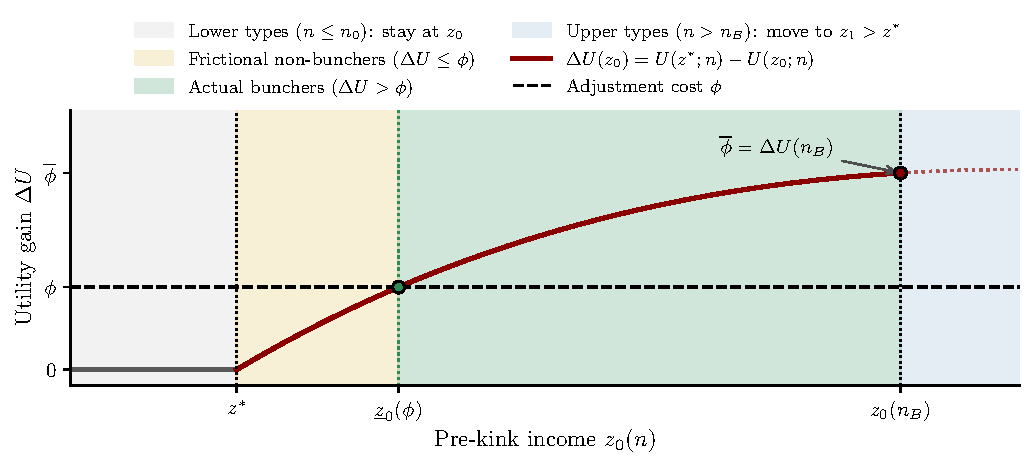
\includegraphics[width=\textwidth]{p2_friction_regimes.pdf}
\caption{Three regimes under optimization frictions ($\phi > 0$) across pre-kink income $z_0(n)$. Lower types ($n \le n_0$, gray) optimally remain at their pre-kink contract ($\Delta U = 0$). Within the potential bunching band $(z^*, z_0(n_B)]$, gross utility gains $\Delta U(z_0)$ (solid crimson curve) increase strictly with $z_0$ up to $\overline{\phi} = \Delta U(n_B)$; agents below the indifference threshold $\underline{z}_0(\phi)$ remain stuck at $z_0$ (yellow region, $\Delta U \le \phi$), whereas agents above $\underline{z}_0(\phi)$ overcome the adjustment cost and bunch at $z^*$ (green region, $\Delta U > \phi$). Upper types ($n > n_B$, blue) adjust toward $z_1(n) > z^*$ rather than $z^*$.}
\label{fig:p2_friction_regimes}
\end{figure}


To characterize which subset of potential bunchers overcomes the adjustment cost $\phi$, we want to express the gross utility gain $\Delta U$ solely as a function of observable pre-kink income $z_0 \equiv z_0(n) \in (z^*, z_0(n_B)]$, eliminating unobserved ability $n$. Recall from the frictionless baseline~\eqref{eq:p2_z0} that optimal pre-kink income satisfies $z_0 = n(1-\tau_0)^\epsilon$. Solving this optimality condition for the ability parameter gives
\begin{equation}
n = z_0 (1-\tau_0)^{-\epsilon}
\qquad \Longleftrightarrow \qquad
n^{-1/\epsilon} = (1-\tau_0)\,z_0^{-1/\epsilon}.
\label{eq:p2_n_inv}
\end{equation}

We now evaluate the piecewise objective $U(z; n) = c(z) - \frac{n^{-1/\epsilon}}{1 + 1/\epsilon}\,z^{1 + 1/\epsilon}$ at the two relevant choices for a potential buncher: remaining passive at $z_0 > z^*$ versus relocating to $z^*$. First, substituting the upper-bracket consumption branch $c(z_0) = (1-\tau_0)z^* + (1-\tau_1)(z_0 - z^*)$ together with~\eqref{eq:p2_n_inv} into $U(z_0; n)$ gives the utility of staying at the old contract:
\begin{align}
U(z_0; n) &= (1-\tau_0)z^* + (1-\tau_1)(z_0 - z^*) - \frac{(1-\tau_0)z_0^{-1/\epsilon}}{1 + 1/\epsilon}\,z_0^{1 + 1/\epsilon} \nonumber\\
&= (1-\tau_0)z_0 - (\tau_1 - \tau_0)(z_0 - z^*) - \frac{\epsilon(1-\tau_0)}{1 + \epsilon}\,z_0 \nonumber\\
&= \frac{1-\tau_0}{1 + \epsilon}\,z_0 - (\tau_1 - \tau_0)(z_0 - z^*).
\label{eq:p2_U_stay}
\end{align}


Second, evaluating the objective at the kink $z^*$---where $c(z^*) = (1-\tau_0)z^*$---and again substituting~\eqref{eq:p2_n_inv} yields the gross utility of relocating to the threshold (before subtracting $\phi$):
\begin{align}
U(z^*; n) &= (1-\tau_0)z^* - \frac{(1-\tau_0)z_0^{-1/\epsilon}}{1 + 1/\epsilon}\,(z^*)^{1 + 1/\epsilon} \nonumber\\
&= (1-\tau_0)z^* - \frac{\epsilon(1-\tau_0)}{1 + \epsilon}\,z_0 \left(\frac{z^*}{z_0}\right)^{1 + 1/\epsilon}.
\label{eq:p2_U_move}
\end{align}
Subtracting~\eqref{eq:p2_U_stay} from~\eqref{eq:p2_U_move} cancels unobserved ability $n$ completely and expresses the gross utility gain solely in terms of $z_0$:
\begin{equation}
\Delta U(z_0) = (\tau_1 - \tau_0)(z_0 - z^*) - (1-\tau_0)\left[\frac{z_0}{1 + \epsilon} - z^* + \frac{\epsilon}{1 + \epsilon}\,z_0\left(\frac{z^*}{z_0}\right)^{1 + 1/\epsilon}\right].
\label{eq:p2_DeltaU}
\end{equation}
Economically, the first term measures the tax savings gained by avoiding the higher rate $\tau_1$ on the excess earnings $(z_0 - z^*)$, whereas the bracketed term captures the net curvature loss from distorting hours away from the pre-kink optimum.

Next, we verify that $\Delta U(z_0)$ is strictly increasing across the bunching band, which guarantees that active bunchers form a single contiguous interval rather than a fragmented set. To differentiate the last term in~\eqref{eq:p2_DeltaU}, rewrite it as $z_0(z^*/z_0)^{1 + 1/\epsilon} = (z^*)^{1 + 1/\epsilon} z_0^{-1/\epsilon}$, whose derivative with respect to $z_0$ is
\begin{equation}
\frac{d}{dz_0}\!\left[z_0\left(\frac{z^*}{z_0}\right)^{1 + 1/\epsilon}\right]
= -\frac{1}{\epsilon}(z^*)^{1 + 1/\epsilon} z_0^{-1/\epsilon - 1}
= -\frac{1}{\epsilon}\left(\frac{z^*}{z_0}\right)^{1 + 1/\epsilon}.
\end{equation}
Applying this identity when differentiating~\eqref{eq:p2_DeltaU} yields the marginal utility gain with respect to pre-kink income:
\begin{equation}
\frac{d\,\Delta U}{dz_0} = (\tau_1 - \tau_0) - \frac{1-\tau_0}{1+\epsilon}\left[1 - \left(\frac{z^*}{z_0}\right)^{1 + 1/\epsilon}\right].
\label{eq:p2_dDeltaU}
\end{equation}

To prove that~\eqref{eq:p2_dDeltaU} is strictly positive on $[z^*, z_0(n_B)]$, define the net-of-tax rate ratio
\begin{equation}
r \equiv \frac{1-\tau_1}{1-\tau_0} \in (0, 1),
\qquad \text{so that} \qquad
\tau_1 - \tau_0 = (1-\tau_0)(1 - r).
\end{equation}
From the marginal buncher's counterfactual income~\eqref{eq:p2_z0nB}, we know that $\frac{z^*}{z_0(n_B)} = r^\epsilon$. Because $z_0 \le z_0(n_B)$ throughout the bunching band, it follows that $\frac{z^*}{z_0} \ge r^\epsilon$, and raising both sides to the positive power $1 + 1/\epsilon$ gives
\begin{equation}
\left(\frac{z^*}{z_0}\right)^{1 + 1/\epsilon} \ge r^{1+\epsilon}.
\end{equation}
Substituting this lower bound and $\tau_1 - \tau_0 = (1-\tau_0)(1 - r)$ into~\eqref{eq:p2_dDeltaU} bounds the derivative from below:
\begin{equation}
\frac{d\,\Delta U}{dz_0} \ge (1-\tau_0)\left[(1 - r) - \frac{1 - r^{1+\epsilon}}{1 + \epsilon}\right] \equiv (1-\tau_0)\,\psi(r).
\end{equation}
Finally, inspect the auxiliary function $\psi(r)$ on $(0, 1)$: at the upper endpoint $r = 1$ we have $\psi(1) = 0$, while its derivative satisfies
\begin{equation}
\psi'(r) = -1 + r^\epsilon < 0 \qquad \text{for all } r \in (0, 1) \text{ and } \epsilon > 0.
\end{equation}
Since $\psi(r)$ decreases strictly to zero as $r \to 1^-$, we must have $\psi(r) > 0$ for every $r \in (0, 1)$. Consequently, $\frac{d\,\Delta U}{dz_0} > 0$ strictly across the entire interval $[z^*, z_0(n_B)]$.\marginnote{Agents with $z_0$ closest to $z^*$ experience only a negligible gain from moving to $z^*$ and therefore fail to pay $\phi$; only higher-income bunchers further up in $(z^*, z_0(n_B)]$ re-optimize.}


Since $\Delta U(z_0)$ is continuous and strictly increasing on $[z^*, z_0(n_B)]$ with $\Delta U(z^*) = 0$, the gain from re-optimizing is largest for the marginal buncher at $z_0(n_B)$. This defines the critical friction threshold $\overline{\phi}$ above which bunching vanishes completely:
\begin{equation}
\overline{\phi} \equiv \Delta U\big(z_0(n_B)\big)
= (\tau_1 - \tau_0)\big(z_0(n_B) - z^*\big) - (1-\tau_0)\left[\frac{z_0(n_B)}{1+\epsilon} - z^* + \frac{\epsilon}{1+\epsilon}\,z_0(n_B)\,r^{1+\epsilon}\right] > 0.
\label{eq:p2_phibar}
\end{equation}
By the Intermediate Value Theorem and strict monotonicity of $\Delta U$, the adjustment cost $\phi$ partitions potential bunchers into two cases:
\begin{itemize}
    \item If $\phi \ge \overline{\phi}$, even the marginal buncher's utility gain falls short of the adjustment cost ($\Delta U(z_0) \le \phi$ for all $z_0 \in (z^*, z_0(n_B)]$), so nobody renegotiates to $z^*$ and $B(\phi) = 0$.
    \item If $0 \le \phi < \overline{\phi}$, there exists a unique lower indifference threshold $\underline{z}_0(\phi) \in [z^*, z_0(n_B))$ implicitly defined by
    \begin{equation}
    \Delta U\big(\underline{z}_0(\phi)\big) = \phi,
    \label{eq:p2_z0_phi_implicit}
    \end{equation}
    satisfying $\underline{z}_0(0) = z^*$ and $\underline{z}_0'(\phi) = \big[\Delta U'(\underline{z}_0(\phi))\big]^{-1} > 0$. Agents in the lower sub-band $z_0 \in \big(z^*, \underline{z}_0(\phi)\big]$ remain stuck at their pre-kink income $z_0 > z^*$, whereas agents in the upper sub-band $z_0 \in \big(\underline{z}_0(\phi), z_0(n_B)\big]$ pay $\phi$ and bunch at $z^*$.
\end{itemize}
Integrating our constant counterfactual density~\eqref{eq:p2_gz} over the active re-optimization interval yields excess mass as a decreasing function of $\phi$:
\begin{equation}
B(\phi) = \begin{cases}
\displaystyle \int_{\underline{z}_0(\phi)}^{z_0(n_B)} g(v)\,dv = g(z^*)\,\big[z_0(n_B) - \underline{z}_0(\phi)\big] & \text{if } 0 \le \phi < \overline{\phi}, \\[8pt]
0 & \text{if } \phi \ge \overline{\phi}.
\end{cases}
\label{eq:p2_B_phi}
\end{equation}

Because~\eqref{eq:p2_z0_phi_implicit} defines $\underline{z}_0(\phi)$ only implicitly, we derive a second-order approximation around $z_0 = z^*$ to build intuition for how $\overline{\phi}$ and $B(\phi)$ scale when the tax jump $\Delta\tau \equiv \tau_1 - \tau_0$ is small. Denote the bracketed disutility term in~\eqref{eq:p2_DeltaU} by
\begin{equation}
h(z_0) \equiv \frac{z_0}{1+\epsilon} - z^* + \frac{\epsilon}{1+\epsilon}\,z_0^{-1/\epsilon}(z^*)^{1+1/\epsilon}.
\end{equation}
Direct differentiation gives
\begin{align}
h'(z_0) &= \frac{1}{1+\epsilon}\left[1 - \left(\frac{z^*}{z_0}\right)^{1+1/\epsilon}\right], &
h''(z_0) &= \frac{1}{\epsilon}\frac{(z^*)^{1+1/\epsilon}}{z_0^{2+1/\epsilon}},
\end{align}
so evaluating at $z_0 = z^*$ yields $h(z^*) = 0$, $h'(z^*) = 0$, and $h''(z^*) = \frac{1}{\epsilon z^*}$. Thus $h(z_0) = \frac{1}{2\epsilon z^*}(z_0 - z^*)^2 + \mathcal{O}\!\big((z_0 - z^*)^3/(z^*)^2\big)$, reducing~\eqref{eq:p2_DeltaU} to the quadratic approximation
\begin{equation}
\Delta U(z_0) \approx (\tau_1 - \tau_0)(z_0 - z^*) - \frac{1-\tau_0}{2\epsilon z^*}(z_0 - z^*)^2.
\label{eq:p2_DeltaU_quad}
\end{equation}
Evaluating~\eqref{eq:p2_DeltaU_quad} at the first-order frictionless bunching width $\Delta z^* \equiv z_0(n_B) - z^* \approx \frac{\epsilon z^*(\tau_1 - \tau_0)}{1 - \tau_0}$ delivers the maximum utility gain
\begin{equation}
\overline{\phi} \approx \frac{1}{2}\,\epsilon\,z^*\,\frac{(\tau_1 - \tau_0)^2}{1 - \tau_0},
\label{eq:p2_phibar_approx}
\end{equation}
confirming that the gains from re-optimizing at a kink scale \emph{quadratically} in the tax jump $\Delta\tau = \tau_1 - \tau_0$ \parencite{chetty2011adjustment}. Setting~\eqref{eq:p2_DeltaU_quad} equal to $\phi < \overline{\phi}$ and selecting the root in $[0, \Delta z^*)$ gives $\underline{z}_0(\phi) - z^* \approx \Delta z^*\big[1 - \sqrt{1 - \phi/\overline{\phi}}\big]$, so~\eqref{eq:p2_B_phi} simplifies to
\begin{equation}
B(\phi) \approx B(0)\sqrt{1 - \frac{\phi}{\overline{\phi}}}, \qquad 0 \le \phi < \overline{\phi}.
\label{eq:p2_B_phi_approx}
\end{equation}


Finally, we evaluate how adjustment frictions distort the empirical elasticity estimator $\hat{\epsilon}(\phi) \equiv \frac{B(\phi)/g(z^*)}{z^*\ln[(1-\tau_0)/(1-\tau_1)]}$. Splitting the total estimation error into its two constituent sources gives
\begin{equation}
\hat{\epsilon}(\phi) - \epsilon
= \underbrace{\big[\hat{\epsilon}(\phi) - \hat{\epsilon}(0)\big]}_{\text{friction bias}}
+ \underbrace{\big[\hat{\epsilon}(0) - \epsilon\big]}_{\text{Taylor approximation error}}.
\label{eq:p2_bias_decomp}
\end{equation}
Combining~\eqref{eq:p2_B_phi} with the frictionless Taylor expansion~\eqref{eq:p2_eps_hat_taylor} reveals why $\hat{\epsilon}(\phi)$ systematically underestimates $\epsilon$:
\begin{enumerate}
    \item \textbf{Friction (attenuation) bias:} For any $0 < \phi < \overline{\phi}$, the inaction threshold satisfies $\underline{z}_0(\phi) > z^*$, so observed excess mass shrinks and the estimator is biased strictly downward:
    \begin{equation}
    \hat{\epsilon}(\phi) - \hat{\epsilon}(0)
    = -\frac{\underline{z}_0(\phi) - z^*}{z^*\ln\!\left(\frac{1-\tau_0}{1-\tau_1}\right)} < 0.
    \label{eq:p2_attenuation_exact}
    \end{equation}
    For $\phi \ge \overline{\phi}$, $B(\phi) = 0$ implies $\hat{\epsilon}(\phi) = 0$ ($100\%$ attenuation, $\hat{\epsilon}(\phi) - \epsilon = -\epsilon$). Under the small-kink approximation~\eqref{eq:p2_B_phi_approx}, $\hat{\epsilon}(\phi) \approx \epsilon\sqrt{1 - \phi/\overline{\phi}}$; for small frictions ($\phi \ll \overline{\phi}$), a first-order expansion in $\phi/\overline{\phi}$ yields
    \begin{equation}
    \hat{\epsilon}(\phi) - \epsilon \approx -\epsilon\,\frac{\phi}{2\overline{\phi}} \approx -\frac{(1-\tau_0)\phi}{z^*(\tau_1 - \tau_0)^2} < 0.
    \end{equation}
    Thus, attenuation bias grows linearly with the utility cost $\phi$ and inversely with the \emph{square} of the tax jump $(\tau_1 - \tau_0)^2$. Small kinks---such as Chile's $4\%$ first bracket---are therefore disproportionately attenuated by adjustment costs relative to large tax reforms \parencite{chetty2011adjustment}.
    \item \textbf{Taylor approximation error:} As established in Part~(i.1), $\hat{\epsilon}(0) - \epsilon = \frac{1}{2}\epsilon^2\ln\!\left(\frac{1-\tau_0}{1-\tau_1}\right) + \mathcal{O}(x^2) > 0$. For small kinks (e.g., $\tau_1 = 0.04$, where $x \approx 0.0408$ and $\frac{1}{2}\epsilon^2 x \sim 10^{-3}$), this small upward linearization error is swamped by the downward attenuation from $\phi > 0$. Overall, $\hat{\epsilon}(\phi)$ acts as a conservative lower bound on the true structural elasticity $\epsilon$ whenever optimization frictions are present.
\end{enumerate}

\subsection*{(ii) Reconstructing the counterfactual density $g(z)$}

Because the counterfactual density $g(z)$ inside the excluded bunching band $[z_L, z_R)$ is fundamentally unobservable, recovering $\hat{B}$ and $\hat{\epsilon}$ requires auxiliary identifying restrictions linking observed counts outside $[z_L, z_R)$ to the missing interior shape. Below we develop two nonparametric alternatives to the global polynomial specification used in Section~1.

\subsubsection*{1. Two alternative strategies to recover $g(z)$}

\paragraph{Alternative 1: Shifted-kink / reference-distribution difference-in-bunching.}
Rather than extrapolating a parametric polynomial across $[z_L, z_R)$, one can exploit an external reference density $h_{\text{ref}}(z)$ observed in a setting where no tax kink operates inside $[z_L, z_R)$—for example, a prior year before nominal bracket indexation moved the statutory cutoff into $[z_L, z_R)$, or an untreated comparison group facing a locally linear schedule. Suppose that in the absence of the kink, the target counterfactual $g_t(z)$ relates to $h_{\text{ref}}(z)$ through a scale-and-shift transformation:
\begin{equation}
\hat{g}^{\mathrm{ref}}(z) = \alpha\,\gamma(z)\,h_{\mathrm{ref}}\!\left(\frac{z}{\lambda}\right),
\label{eq:p2_alt1}
\end{equation}
where $\lambda > 0$ adjusts for aggregate nominal wage growth or inflation between the reference and target regimes, $\alpha > 0$ normalizes total mass, and $\gamma(z)$ is a low-order smooth tilt function (e.g., $\gamma(z) = \exp(\delta_0 + \delta_1 z)$ or $\gamma(z) \equiv 1$ in the pure proportional case) fitted solely on the uncontaminated exterior bins $z \notin [z_L, z_R)$ (with iterative right-tail reweighting for missing mass when appropriate).
\begin{itemize}
    \item \emph{Justification:} Actual earnings distributions often exhibit institutional focal points, round-number heaping, and non-polynomial curvature that global polynomials smooth over. Anchoring $g(z)$ to $h_{\text{ref}}(z)$ preserves these genuine empirical features inside $[z_L, z_R)$.
    \item \emph{Identifying assumptions:} (A1) \emph{No kink distortion in the reference group/period} on $[z_L/\lambda,\, z_R/\lambda)$; (A2) \emph{Rank/shape invariance}, meaning any macroeconomic shift between the reference and target regimes affects the distribution smoothly through $(\alpha, \lambda, \gamma(z))$ without idiosyncratic shocks concentrated inside $[z_L, z_R)$; and (A3) \emph{No intertemporal anticipation or spillover} across regimes.
\end{itemize}

\paragraph{Alternative 2: Deep generative density estimation via censored Normalizing Flows.}
Instead of fitting an ad-hoc global polynomial or requiring an external untreated sample, one can model the counterfactual density using a \emph{Normalizing Flow} \parencite{rezende2015variational,papamakarios2021normalizing}—a deep generative model that parameterizes a flexible, smooth, and strictly invertible diffeomorphism $T_\theta : \mathbb{R}_{++} \to \mathbb{R}$ (implemented, for instance, as a composition of monotonic rational-quadratic neural splines, \parencite{durkan2019neural}) mapping counterfactual income $z$ into a standard normal latent variable $u = T_\theta(z) \sim p_U(u) = \mathcal{N}(0, 1)$.\marginnote{Unlike global polynomials, monotonic spline normalizing flows guarantee positivity ($g_\theta(z) > 0$), exact probability normalization, and $C^1$-smooth interpolation across $[z_L, z_R)$ without Runge oscillations in the tails.} By the change-of-variables theorem, the implied counterfactual density is given in closed form by
\begin{equation}
g_\theta(z) = p_U\big(T_\theta(z)\big)\left|\frac{\partial T_\theta(z)}{\partial z}\right|.
\label{eq:p2_nf_density}
\end{equation}
Because observations inside $[z_L, z_R)$ are contaminated by bunching and missing mass, $T_\theta$ cannot be trained by standard maximum likelihood over the full support. Instead, we estimate $\theta$ by maximizing the \emph{censored (truncated) conditional log-likelihood} over the uncontaminated exterior region $\mathcal{O} \equiv [z_l, z_r] \setminus [z_L, z_R)$:
\begin{equation}
\mathcal{L}(\theta) = \sum_{i : z_i \in \mathcal{O}} \left[ \ln p_U\big(T_\theta(z_i)\big) + \ln\left|\frac{\partial T_\theta(z_i)}{\partial z}\right| - \ln\!\Big(1 - \big[F_U\big(T_\theta(z_R)\big) - F_U\big(T_\theta(z_L)\big)\big]\Big) \right],
\label{eq:p2_nf_loss}
\end{equation}
where $F_U(\cdot)$ denotes the standard normal CDF and the third term normalizes the likelihood by the probability mass assigned outside the excluded interval (with iterative right-tail reweighting applied to upper-bracket observations $z_i \ge z_R$ to account for displaced mass). Figure~\ref{fig:p2_nf_mechanism} illustrates this generative mechanism intuitively: a smooth, strictly increasing transformation $T_\theta^{-1}$ maps a simple standard normal latent variable $u$ into the skewed counterfactual earnings distribution $g_\theta(z)$, interpolating across the censored band $[z_L, z_R)$ solely from the shape learned in the exterior data.
\begin{figure}[htbp]
\centering
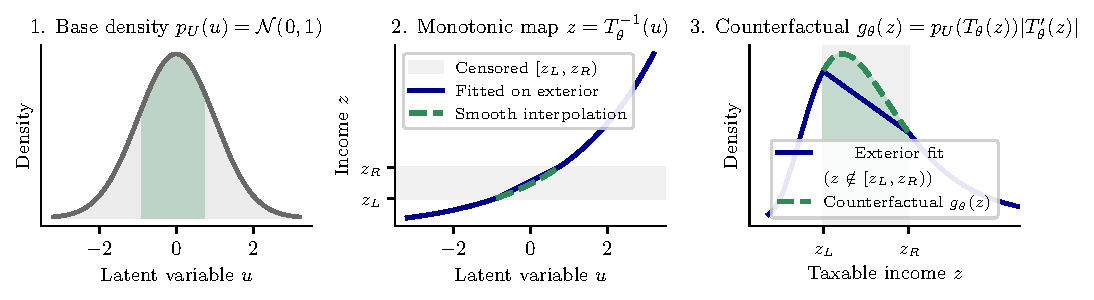
\includegraphics[width=\textwidth]{p2_nf_mechanism.pdf}
\caption{Illustration of a censored Normalizing Flow (adapted from \parencite{papamakarios2021normalizing}). Left: standard normal latent density $p_U(u)$. Center: smooth, strictly increasing spline map $z = T_\theta^{-1}(u)$ trained on exterior observations ($z \notin [z_L, z_R)$). Right: resulting counterfactual income density $g_\theta(z)$, which smoothly interpolates across the censored region $[z_L, z_R)$.}
\label{fig:p2_nf_mechanism}
\end{figure}

When individual covariates $X_i$ (such as age, industry, or gender) are observed, conditioning the spline parameters on $X_i$ yields a \emph{Conditional Normalizing Flow} $T_\theta(z; X_i)$ \parencite{trippe2018conditional,winkler2019learning}, whose marginal counterfactual density is recovered by integrating $g_\theta(z \mid X_i)$ over the empirical covariate distribution. Moreover, training a deep ensemble $\{\theta^{(m)}\}_{m=1}^M$ across random initializations and spline knot placements generates a family of admissible counterfactual curves $\{g_{\theta^{(m)}}(z)\}_{m=1}^M$ and a corresponding interval of elasticities $[\hat{\epsilon}_{\min}, \hat{\epsilon}_{\max}]$.
\begin{itemize}
    \item \emph{Justification:} Normalizing flows are universal density approximators that capture heavy right tails, skewness, and local curvature in administrative earnings data while automatically enforcing non-negativity ($g_\theta(z) > 0$) and unit-mass integration without high-degree polynomial boundary artifacts.
    \item \emph{Identifying assumptions:} (B1) \emph{Localized kink distortion}, so observations in $\mathcal{O} = [z_l, z_r] \setminus [z_L, z_R)$ (after right-tail mass adjustment) are generated by the true counterfactual distribution; (B2) \emph{Smooth transport regularity} ($C^1$ diffeomorphism), ruling out abrupt latent jumps or kinks in the base-to-income map inside $[z_L, z_R)$; and (B3) \emph{Out-of-support interpolation stability}, meaning that the inductive bias of the spline architecture (controlled via derivative regularization or weight decay) accurately interpolates the density trajectory across the censored band $[z_L, z_R)$.
\end{itemize}

\subsubsection*{2. Graphical illustration and point estimates vs.\ ranges}

Figure~\ref{fig:p2_counterfactuals} illustrates both counterfactual constructions in the $(z, g(z))$ plane\footnote{\texttt{code: source/plots/p2.py:L71}} alongside an observed density $h(z)$ displaying a sharp bunching spike at $z^*$ and a localized missing-mass deficit just above $z^*$ inside the excluded band $[z_L, z_R)$.

\begin{figure}[htbp]
\centering
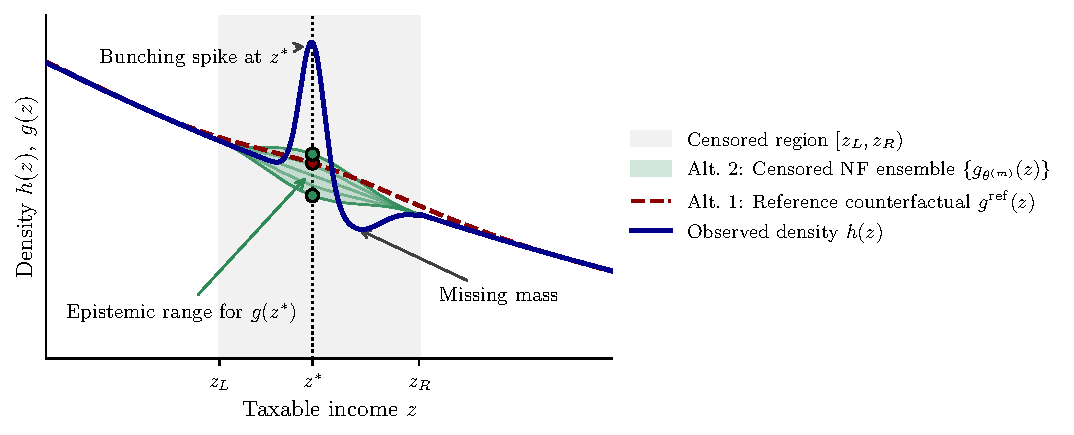
\includegraphics[width=\textwidth]{p2_counterfactual_alternatives.pdf}
\caption{Observed density $h(z)$ around $z^*$ compared with Alternative~1 ($g^{\mathrm{ref}}(z)$) and Alternative~2 (censored Normalizing Flow ensemble $\{g_{\theta^{(m)}}(z)\}$ trained outside $[z_L, z_R)$). Markers at $z^*$ highlight the implied range of counterfactual heights $g(z^*)$.}
\label{fig:p2_counterfactuals}
\end{figure}

As Figure~\ref{fig:p2_counterfactuals} makes clear, we cannot rely on a single point estimate of $\epsilon$ and should instead report an interval of plausible values for three complementary reasons:
\begin{enumerate}
    \item \textbf{Fundamental non-identification of $g(z)$ inside $[z_L, z_R)$:} Because counterfactual behavior at the kink is never observed, every point estimate depends on untestable interpolation or extrapolation choices—such as the polynomial degree, outer fitting window $[z_l, z_r]$, reference period, or neural-spline inductive bias. As demonstrated empirically in Section~1(iv), merely varying the outer polynomial window in Chile shifts $\hat{\epsilon}$ across $[0.1272,\, 0.5271]$, a fourfold span that standard errors from a single specification fail to capture.
    \item \textbf{Epistemic uncertainty across admissible counterfactual models:} Even flexible universal approximators such as censored Normalizing Flows are only constrained by data outside $[z_L, z_R)$. Multiple smooth diffeomorphisms $T_{\theta^{(m)}}$ can achieve virtually identical exterior log-likelihoods on $\mathcal{O}$ while interpolating slightly different trajectories across the censored region, yielding a range of baseline heights $g_{\theta^{(m)}}(z^*)$. Collapsing this epistemic set to a single point estimate creates false precision.
    \item \textbf{Compounding uncertainty from optimization frictions:} As established in Part~(i.2), adjustment costs ($\phi > 0$) attenuate $\hat{\epsilon}(\phi)$ below the structural elasticity $\epsilon$, whereas counterfactual curvature misspecification can bias $\hat{\epsilon}$ in either direction. Reporting an identified range—combining sensitivity across alternative counterfactual estimators and friction bounds—provides policymakers with transparent lower and upper bounds for revenue and welfare projections.
\end{enumerate}
